
The exponential distribution is memoryless and its development in time will therefore not depend on its starting point. As the sojourn times are independet of each other and exponentially distributed, the sojourn time in a given state therefore will not depend on which states you have visited earlier. Thus $\{X(t):t \geq 0 \}$  satisfies the Markov property 

$$P(X(t+s)=j|X(s)=i, X(u), 0 \leq u \leq s)=P(X(t+s)=j|X(s)=j)$$ 
for $i,j = 0,1,...$ and for all $s \geq 0$ and $t >0 $.

The jump probabilities are $P(S \rightarrow I_L)= 1 - \alpha$, $P(S \rightarrow I_H)= \alpha$, $P(I_L \rightarrow S)= P(I_H \rightarrow S) = 1$ and $P(I_L \rightarrow I_H)= P(I_H \rightarrow I_L) = 0$. Using $\alpha = 0.10$, $P(S \rightarrow I_L)= 0.9$ and $P(S \rightarrow I_H)= 0.1$. 

The transition rates are found from formula $q_{ij} = P(i \rightarrow j ) q_i$, where $q_i = \sum_{j \neq i} q_{ij}$. The rates are then expressed as $q_{SL} = (1-\alpha)\lambda $, $q_{SH} = \alpha \lambda$, $q_{LS} = 1/\mu_L$ and $q_{HS} = 1/\mu_H$. Using $\alpha = 0.10$ and inserting the values of $\lambda$, $\mu_L$ and $\mu_H$, the transition rates are 
$$q_{SL} = 0.009,\text{ } q_{SH} = 0.001, \text{ } q_{LS} = 1/7, \text{ } q_{HS} = 1/20 \text{ and } q_{HL}=q_{LH}=0.$$

The transition diagram of $\{X(t):t \geq 0 \}$ is illustrated in figure \ref{transdiagramA}. 

\begin{figure}
    \centering
    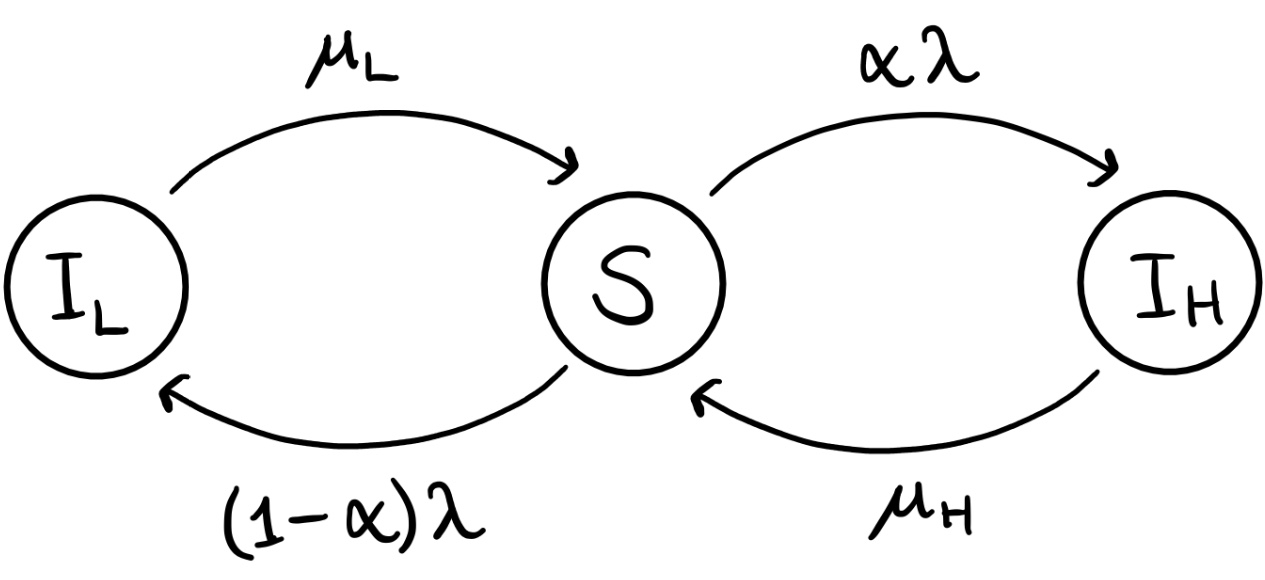
\includegraphics[width=90mm]{TransDiag1A.png}
    \caption{Transition diagram of $\{X(t):t\geq0\}$.}
    \label{transdiagramA}
\end{figure}




